\documentclass[10pt]{article}

\usepackage[letterpaper,top=0.68in,bottom=0.72in,left=0.67in,right=0.67in,columnsep=0.23in]{geometry}
\usepackage[T1]{fontenc}
\usepackage[utf8]{inputenc}
\usepackage{newtxtext,newtxmath}
\usepackage{microtype}
\usepackage{amsmath,mathtools}
\usepackage{booktabs}
\usepackage{multirow}
\usepackage{graphicx}
\usepackage{subcaption}
\usepackage{xcolor}
\usepackage{listings}
\usepackage[most]{tcolorbox}
\usepackage[numbers,sort&compress]{natbib}
\usepackage[colorlinks=true,allcolors=blue]{hyperref}
\usepackage{url}
\usepackage{enumitem}
\usepackage{balance}
\usepackage{titlesec}
\usepackage{array}

\setlength{\parindent}{1em}
\setlength{\parskip}{0pt}
\setlength{\textfloatsep}{7pt plus 2pt minus 2pt}
\setlength{\floatsep}{6pt plus 2pt minus 2pt}
\setlength{\intextsep}{6pt plus 2pt minus 2pt}
\setlength{\abovecaptionskip}{3pt}
\setlength{\belowcaptionskip}{-2pt}
\emergencystretch=2em
\Urlmuskip=0mu plus 2mu
\captionsetup{font=small,labelfont=bf}
\setlist[itemize]{leftmargin=1.2em,itemsep=1pt,topsep=2pt}
\setlist[enumerate]{leftmargin=1.35em,itemsep=1pt,topsep=2pt}
\titleformat{\section}{\large\bfseries}{\thesection}{0.52em}{}
\titlespacing*{\section}{0pt}{8pt}{3.5pt}
\titleformat{\subsection}{\normalsize\bfseries}{\thesubsection}{0.45em}{}
\titlespacing*{\subsection}{0pt}{5.5pt}{2pt}

\newcommand{\method}{\textsc{Audio-LF-CBM}}
\newcommand{\R}{\mathbb{R}}
\newcommand{\best}[1]{\textbf{#1}}

% Prompt boxes used in Appendix~\ref{app:prompt-templates}.
\definecolor{anon}{RGB}{80,80,80}
\lstdefinestyle{mystyle}{
   breaklines=true,
   basicstyle=\scriptsize\ttfamily,
   numbers=none,
   language={},
   framextopmargin=0pt,
   framexbottommargin=0pt,
   breakindent=0pt,
   showspaces=false,
   keywordstyle=\bfseries,
   showstringspaces=false,
   columns=fullflexible,
   morekeywords={Style, Consistency, Accuracy, Ethics, Score}
}

\newtcblisting{prompt}[2][]{
   arc=3pt, outer arc=3pt,
   width=\linewidth,
   left=1mm,
   top=0mm,
   bottom=0mm,
   title=#2,
   colback=gray!5!white,
   colframe=black!75!black,
   fonttitle=\bfseries,
   listing only,
   listing options={style=mystyle},
   breakable,
   #1
}

\newtcblisting{inference}[2][]{
   arc=3pt, outer arc=3pt,
   width=\linewidth,
   left=1mm,
   top=0mm,
   bottom=0mm,
   title=#2,
   colback=red!5!white,
   colframe=red,
   fonttitle=\bfseries,
   listing only,
   listing options={style=mystyle},
   breakable,
   #1
}

\newtcblisting{anonymize}[2][]{
   arc=3pt, outer arc=3pt,
   width=\linewidth,
   left=1mm,
   top=0mm,
   bottom=0mm,
   title=#2,
   colback=anon!5!white,
   colframe=anon,
   fonttitle=\bfseries,
   listing only,
   listing options={style=mystyle},
   breakable,
   #1
}

\begin{document}

\twocolumn[
\begin{@twocolumnfalse}
\begin{center}
{\LARGE\bfseries Label-Free Concept Bottleneck Models for Audio:\
Perceptual Vocabularies, Sparse Predictions, and Temporal Explanations\par}
\vspace{0.45em}
{\normalsize
Amine Maazizi$^{1,2,*}$ \qquad Adam Gassem$^{1,2,*}$\\[-1pt]
$^{1}$ENSTA Paris \qquad $^{2}$MVA, ENS Paris-Saclay\\[-1pt]
\texttt{amine.maazizi@ensta.fr} \qquad \texttt{adam.gassem@ensta.fr}\\[-1pt]
$^{*}$Equal contribution.\par}
\end{center}
\vspace{-0.2em}
\noindent\rule{\textwidth}{0.35pt}
\vspace{0.3em}

\begin{abstract}
Concept Bottleneck Models expose human-readable variables but normally require concept annotations. We adapt Label-Free Concept Bottleneck Models (LF-CBMs) from vision to audio by projecting fine-tuned Audio Spectrogram Transformer (AST) features onto CLAP-supervised textual concepts. Audio calls for a different vocabulary from static images: class evidence is often expressed through shared perceptual dimensions such as pitch, harmonicity, roughness, attack, repetition, and reverberation, and it unfolds over time. We therefore augment vanilla class-conditioned LF-CBM concepts with (i) a dataset-independent broad auditory vocabulary and (ii) acoustic dimensions generated jointly for groups of confusable classes. On fixed held-out splits, LF+broad obtains 93.50/93.39 on ESC-50 and 89.84/90.94 on UrbanSound8K (accuracy/macro-F1), matching or exceeding the fine-tuned AST. For CREMA-D, a speech-targeted version of the same LF-CBM pipeline reaches 70.25/51.58, narrowing the gap to AST while retaining 92.79\% sparse-head zeros. Broad concepts improve vanilla LF-CBM accuracy on all three datasets. We additionally support exact test-time edits of concept signals; a coarse top-five intervention corrects 8 of 14 curated ESC-50 errors in the interactive showcase. Finally, applying the same bottleneck to overlapping 1-second windows produces temporal concept trajectories that reveal when interpretable evidence appears and expose failure cases that a single global score hides.
\end{abstract}

\vspace{0.25em}
\noindent\textbf{Keywords:} concept bottleneck models; audio classification; explainable AI; audio--language models; temporal explanations
\vspace{0.25em}
\noindent\rule{\textwidth}{0.35pt}
\vspace{0.55em}
\end{@twocolumnfalse}
]

\section{Introduction}
State-of-the-art audio classifiers can recognize environmental events and speech affect while exposing little about the evidence behind a decision. Their predictions are nevertheless naturally discussed in audible terms: \emph{rapid impacts}, \emph{steady low-frequency hum}, \emph{high-pitched chirps}, or \emph{slow strained speech}. Concept Bottleneck Models (CBMs) make such variables explicit and permit a user to inspect or edit them before class prediction \citep{koh2020concept}. Their usual requirement for concept annotations, however, is impractical for most audio datasets.

Label-Free Concept Bottleneck Models (LF-CBMs) avoid manual annotations by aligning a task backbone with semantic activations from a pretrained vision--language model \citep{oikarinen2023labelfree}. This modular construction suggests an audio counterpart: keep a task-trained audio backbone, replace CLIP with an audio--text teacher, and learn a projection onto textual auditory concepts. We implement this idea with AST \citep{gong2021ast} and CLAP \citep{elizalde2023clap}, then compare the resulting model with the original fine-tuned classifier on three benchmarks.

The transfer is not merely an encoder substitution. Image concepts often name objects, parts, colors, and spatial relations. Audio evidence instead depends strongly on generic perceptual and dynamical axes: pitch, spectral balance, bandwidth, harmonicity, timbre, roughness, continuity, periodicity, attack/decay, modulation, and spatial impression. We hypothesize that broad terms can therefore carry more task information in audio than similarly broad visual adjectives. For example, \emph{high-pitched} directly constrains acoustic frequency content and can distinguish alarms, chirps, or vocalizations; a visual term such as \emph{bright} may conflate illumination, reflectance, and camera exposure and is often less diagnostic of object identity. This is a hypothesis about useful vocabularies, not a claim that generic terms are universally informative.

Audio is also temporal. A sound may be brief, repeated after silence, or masked by a background source. A full-clip concept score answers \emph{what} evidence was present but not \emph{when}. We consequently run the frozen concept projection on overlapping 1-second waveform windows and decompose the predicted-class evidence through time. We evaluate this windowed version as both an explanation tool and a segmented-inference ablation.

\paragraph{Contributions.}
\begin{itemize}
    \item We establish an LF-CBM pipeline for audio and compare it with its fine-tuned AST backbone on ESC-50, UrbanSound8K, and CREMA-D.
    \item We introduce broad perceptual concepts and group-wise contrastive concepts, and isolate their effects through four matched concept-source ablations.
    \item We report accuracy, macro-F1, retained concept counts, and sparse-head support rather than treating a named layer alone as evidence of interpretability.
    \item We demonstrate exact concept-signal interventions that can correct individual errors, and extend explanations temporally with 1-second windows and three pooling rules.
\end{itemize}
Code, checkpoints, and the interactive ESC-50 demo are available in the \href{https://github.com/Adam-Ousse/Label-free-CBM-Audio}{project repository}.

\section{Related Work}
\paragraph{Concept-based prediction.}
CBMs predict annotated concepts before the label, enabling inspection and intervention \citep{koh2020concept}. Later work introduced richer concept embeddings \citep{zarlenga2022cem}, post-hoc conversion of trained networks \citep{yuksekgonul2023posthoc}, and language-model-generated vocabularies \citep{yang2023labo}. LF-CBM learns a linear concept projection from a pretrained representation using multimodal similarity patterns as weak targets \citep{oikarinen2023labelfree}. Because named coordinates can still encode unintended information or behave differently from their labels, predictive performance, sparsity, and intervention behavior should be evaluated separately \citep{margeloiu2021intended,almudevar2025bottleneck}.

\paragraph{Audio--language models and audio explanations.}
CLAP provides a shared audio--text space for zero-shot recognition \citep{elizalde2023clap}, building on systems such as AudioCLIP \citep{guzhov2022audioclip}. Prompt wording and compositional structure materially affect audio--text alignment \citep{ghosh2025reclap,ghosh2024compa}. Recent audio interpretation work includes post-hoc CBM reproduction studies \citep{midavaine2024repro}, sparse CLAP-grounded audio representations \citep{zhang2025audio}, and listenable decompositions based on non-negative matrix factorization \citep{parekh2024nmf}. Our focus is the LF-CBM construction: an automatically generated vocabulary, a task-trained AST representation, CLAP supervision, and a sparse prediction head.

\paragraph{Temporal grounding.}
Static clip-level alignment is weak at temporal order and localization, motivating explicitly temporal audio--language models and benchmarks \citep{timeaudio2025}. Our goal is narrower. We reuse the exact concepts and classifier learned by the global CBM on short windows, producing time-indexed class contributions without training a separate temporal explanation model.

\section{Audio LF-CBM}
\label{sec:method}

\begin{figure*}[t]
\centering
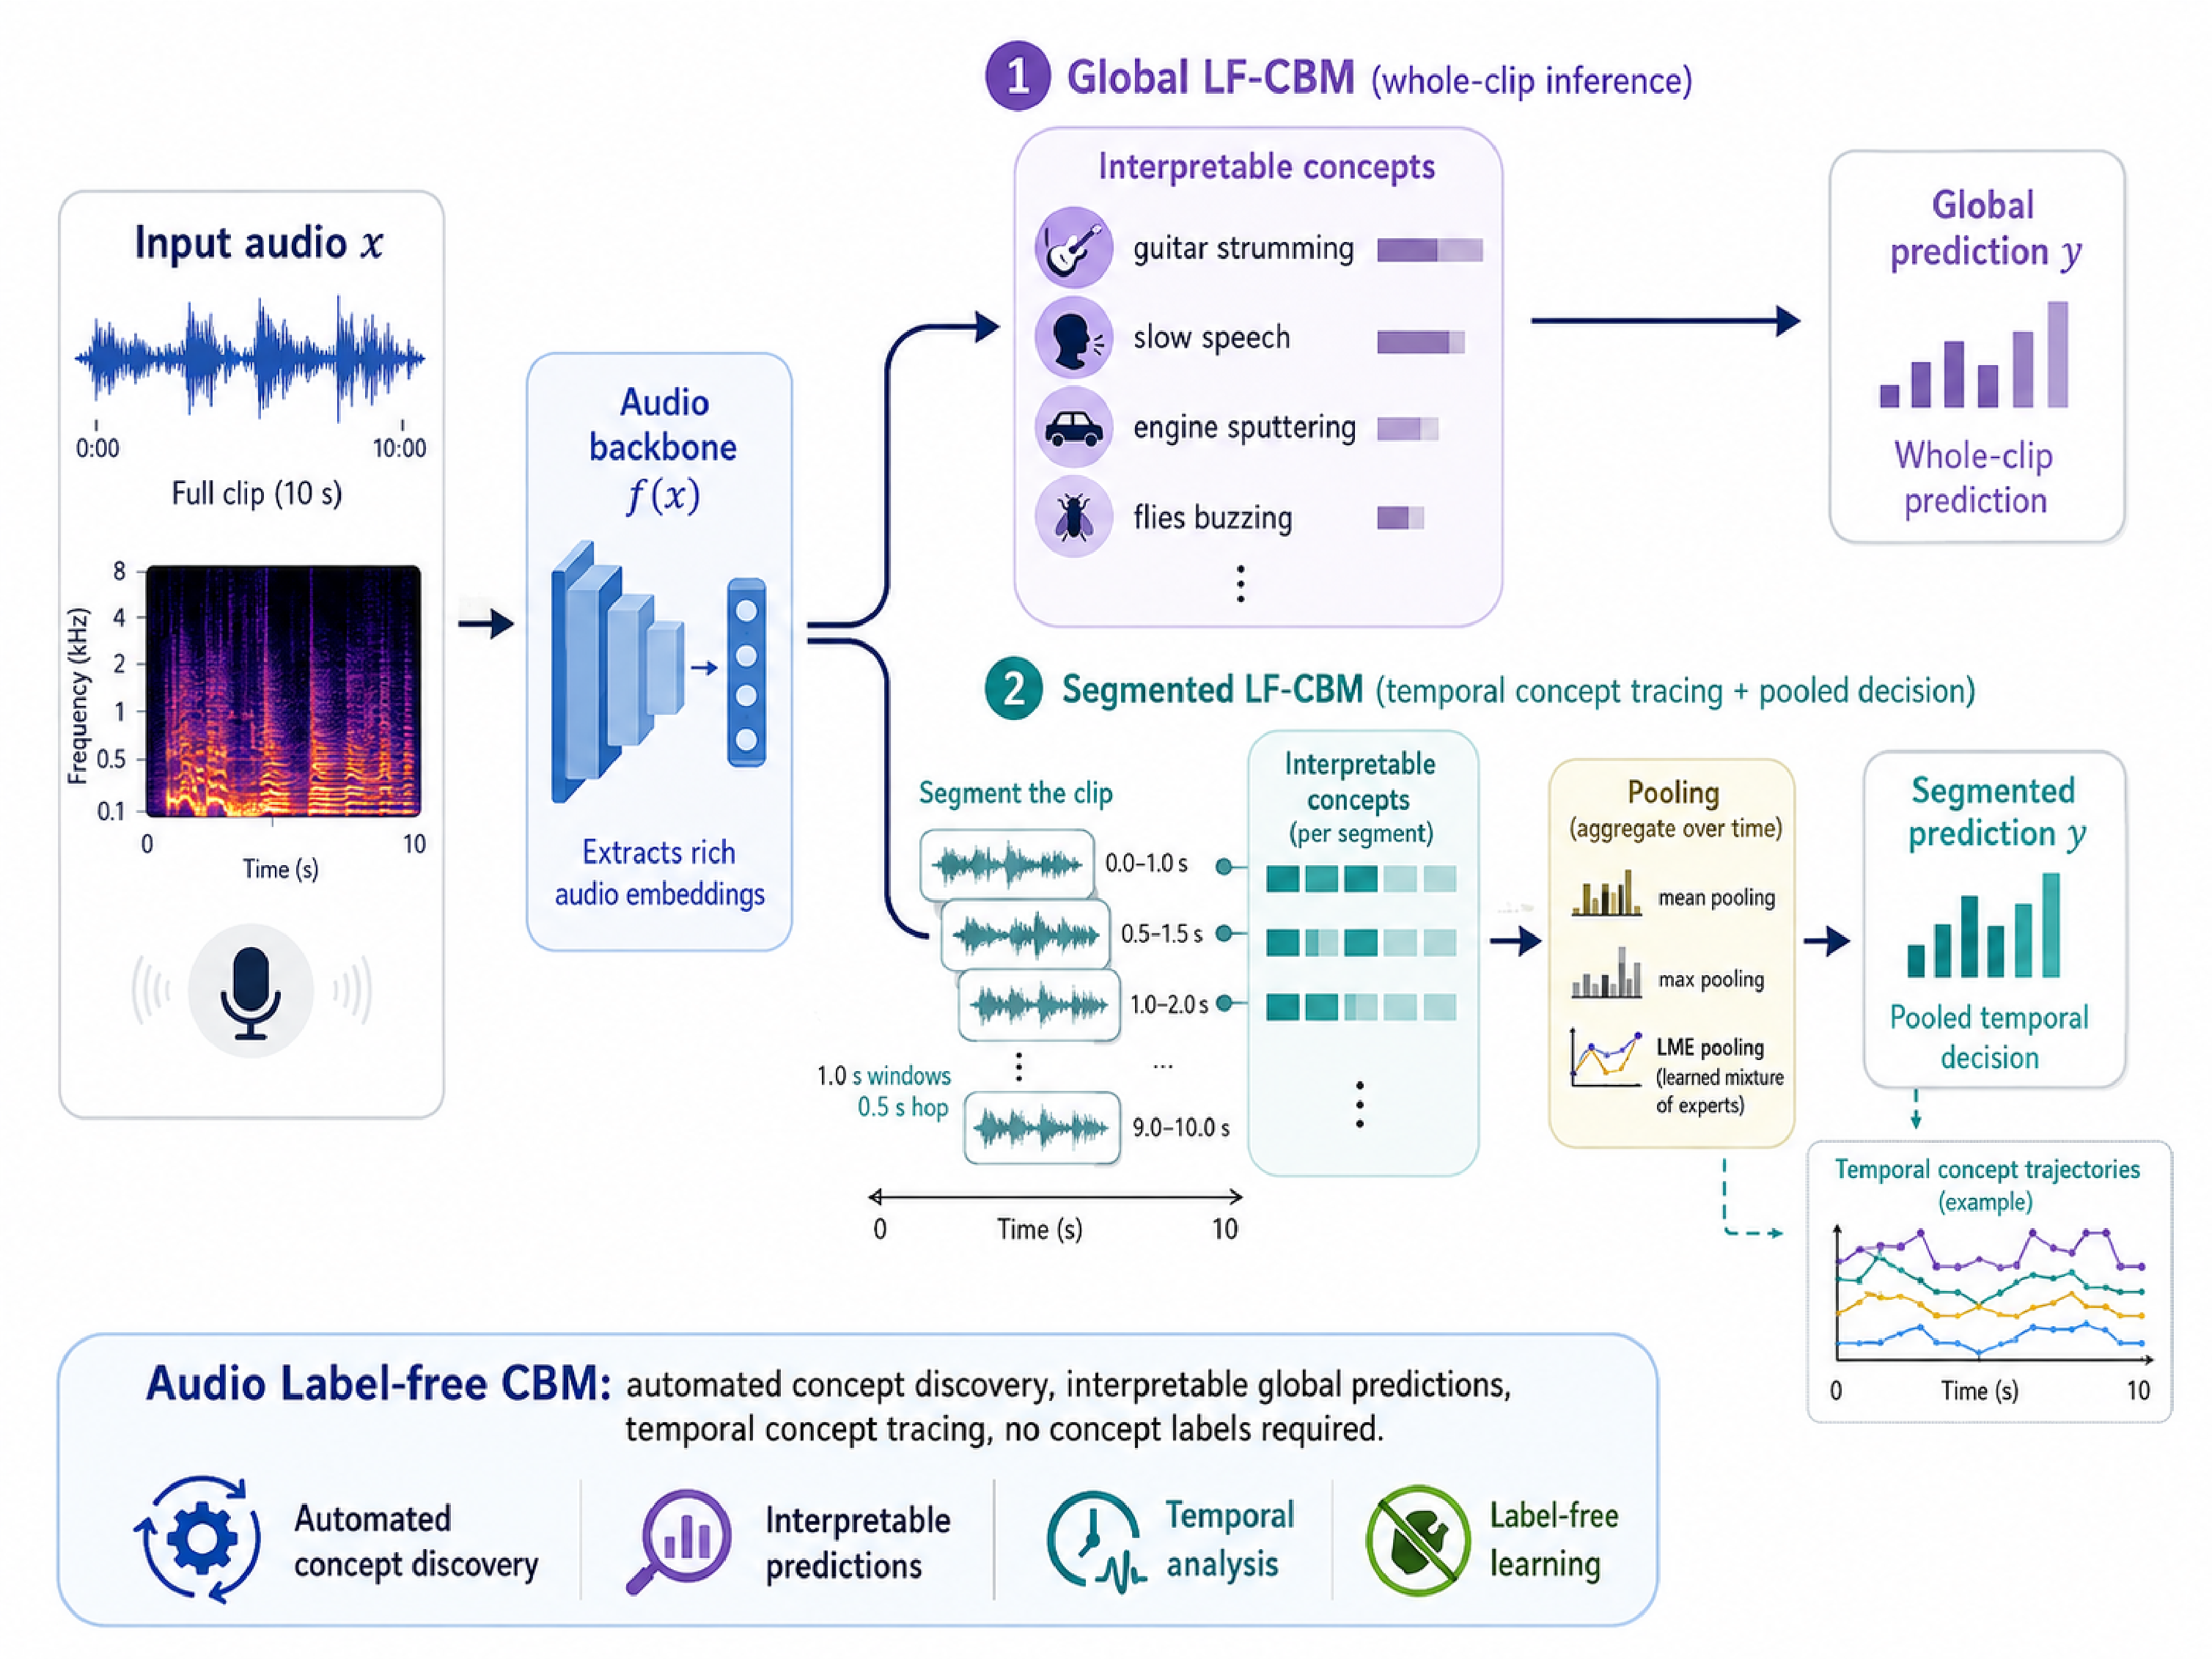
\includegraphics[width=0.6\textwidth]
{media/audio_lf_cbm_architecture.pdf}
\caption{Overview of \method. A fine-tuned AST backbone is projected into a CLAP-supervised concept space, after which a sparse linear head predicts the class from standardized concept activations. The trained bottleneck can also be reused on overlapping audio windows to obtain time-indexed concept contributions without retraining the global model.}
\label{fig:architecture}
\end{figure*}

\subsection{Label-free concept projection}

Figure~\ref{fig:architecture} summarizes the global prediction path and the post-training temporal explanation branch.

Let $D=\{(x_i,y_i)\}_{i=1}^{N}$ be an audio dataset and $C=\{c_j\}_{j=1}^{M}$ a textual concept vocabulary. A frozen fine-tuned AST backbone produces $f(x_i)\in\R^d$. Frozen CLAP audio and text encoders, $E_a$ and $E_t$, define weak concept targets
\begin{equation}
P_{ij}=\cos\!\left(E_a(x_i),E_t(c_j)\right).
\label{eq:clap}
\end{equation}
A learned linear map $W_c\in\R^{M\times d}$ gives the concept vector
\begin{equation}
a(x_i)=W_cf(x_i).
\label{eq:concept}
\end{equation}
As in LF-CBM, each projected concept is trained to match its CLAP activation pattern across examples using the cosine-cubed objective, and concepts with insufficient validation alignment are removed \citep{oikarinen2023labelfree}. We standardize the retained concept activations using training statistics. Finally, an elastic-net linear classifier produces
\begin{equation}
\ell(x_i)=W_Fa(x_i)+b_F,
\qquad r_{ijk}=a_j(x_i)W_{F,kj},
\label{eq:head}
\end{equation}
where $r_{ijk}$ is concept $j$'s signed contribution to class $k$.

\subsection{Three complementary concept sources}
We form the initial candidate vocabulary as
\begin{equation}
\mathcal C_0=\mathcal C_{\mathrm{LF}}\cup\mathcal C_{\mathrm{broad}}\cup\mathcal C_{\mathrm{contrast}}.
\end{equation}
LLM generates all three sources, but never decides whether a concept occurs in a recording.

\paragraph{Vanilla LF concepts.}
For each target class, audio-specific versions of the original LF-CBM prompts request important audible characteristics, common acoustic components, and broader sound-event categories. These candidates are class-associated; for example, \emph{rapid barking} may be associated with \emph{dog}.

\paragraph{Broad perceptual concepts.}
A shared, dataset-independent prompt does not include any target class names. It requests short atomic concepts spanning loudness, pitch, spectral balance, bandwidth, harmonicity, timbre, texture, roughness, continuity, periodicity, rhythm, attack/decay, modulation, impulsiveness, temporal density, reverberation, distance, spatial impression, and production mechanism. It explicitly excludes object identities, event labels, emotions, visual information, and long descriptions. Examples include \emph{high-pitched}, \emph{broadband}, \emph{rough}, \emph{impulsive}, and \emph{slow decay}. The same generated vocabulary is reused across datasets.

\paragraph{Contrastive concepts.}
LLM first groups target classes that may be acoustically confusable; groups overlap, so a class can participate in more than one comparison. It then receives each group jointly and proposes general audible dimensions on which the classes may differ, such as \emph{rapid repetitive impacts}, \emph{steady low-frequency hum}, or \emph{metallic resonance}. Prompts prohibit class names and synonyms. Group-wise generation avoids the redundancy of enumerating every class pair. Figure~\ref{fig:concept_construction} summarizes how the three complementary sources form the four vocabularies evaluated in our ablations.

\begin{figure*}[t]
\centering
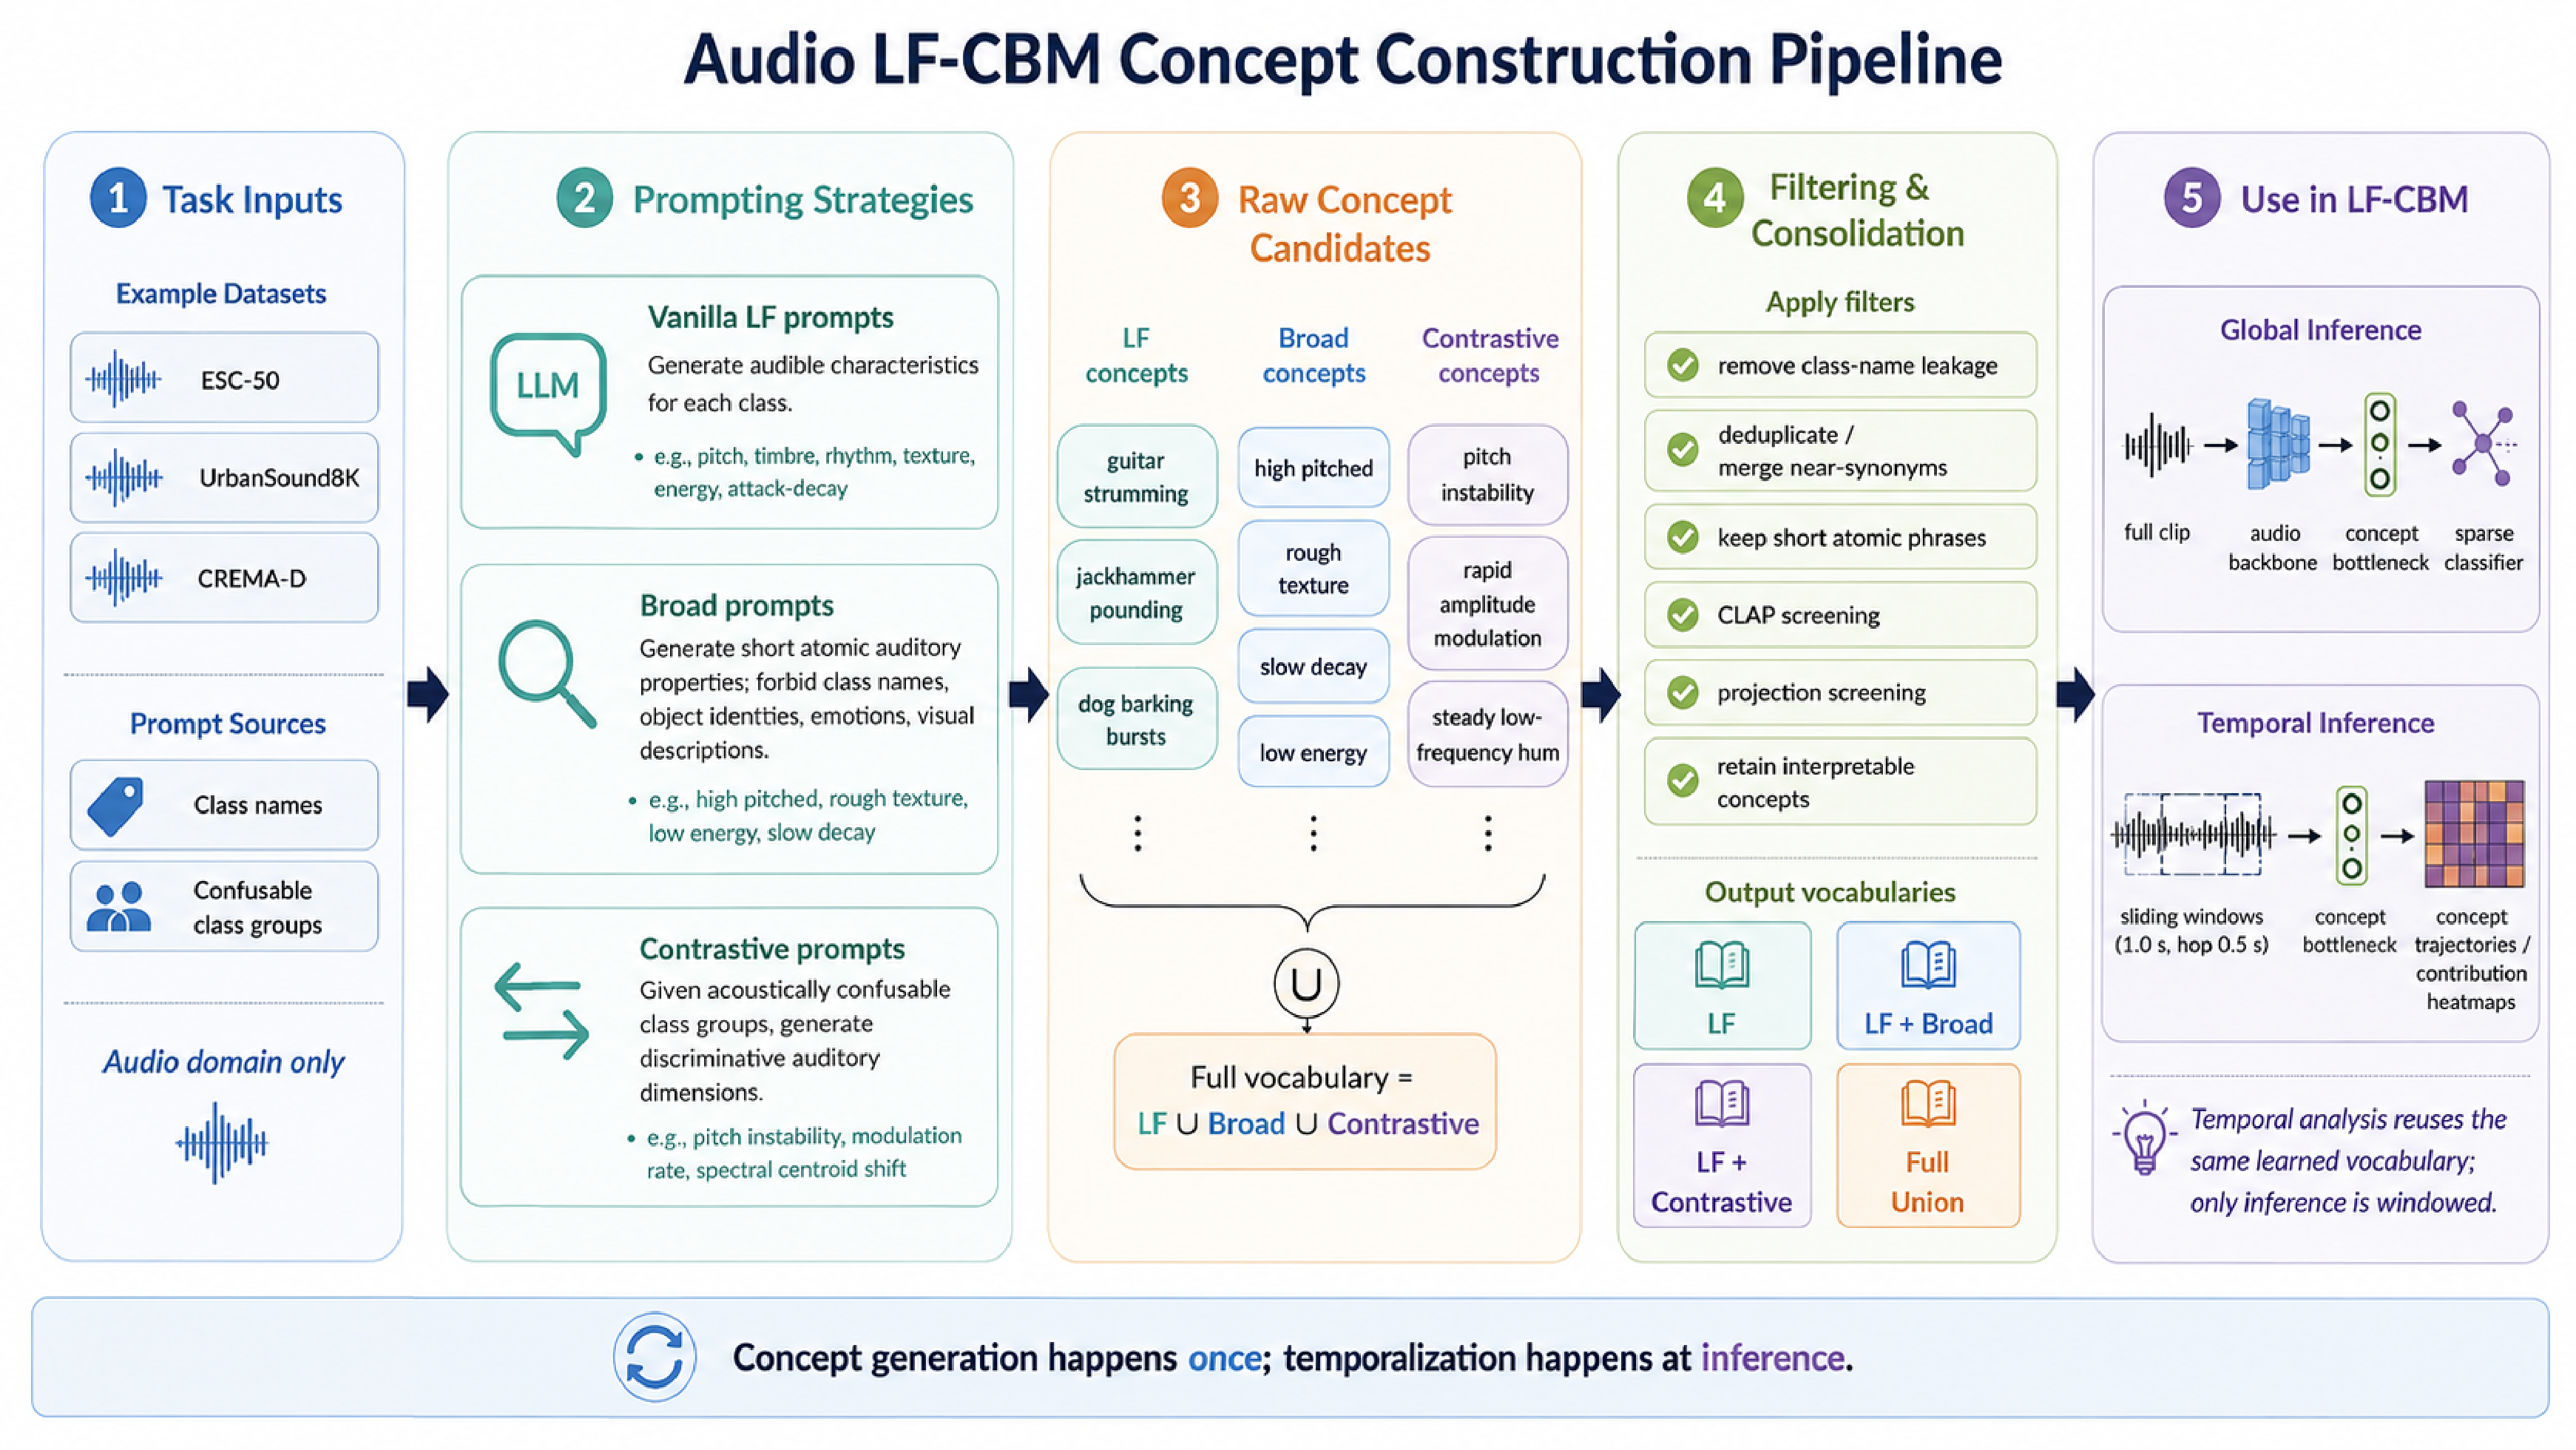
\includegraphics[width=0.6\textwidth]
{media/audio_lf_cbm_concept_construction_pipeline.pdf}
\caption{Construction of the audio concept vocabulary. Vanilla LF concepts provide class-associated semantic candidates, broad concepts introduce dataset-independent perceptual audio attributes, and contrastive concepts target acoustic dimensions separating confusable class groups. The resulting candidates are filtered through the LF-CBM grounding and projectability pipeline before sparse classification.}
\label{fig:concept_construction}
\end{figure*}

\subsection{Filtering and ablation variants}
We reuse the LF-CBM filtering sequence: remove long phrases, class-name matches, and semantic duplicates; remove concepts with insufficient CLAP activation on training audio; learn $W_c$; and remove concepts below the projection-alignment cutoff. The four experimental variants are vanilla LF, LF+broad, LF+contrastive, and the full union. Provenance metadata is retained during generation, while the final flat lists remain compatible with the original training code.

\subsection{Counterfactual concept editing}
The bottleneck permits exact edits without rerunning AST. For displayed concepts $J$ and user-chosen multipliers $\gamma_j$, the edited logits are
\begin{equation}
\ell'_k=\ell_k+\sum_{j\in J}(\gamma_j-1)a_jW_{F,kj}.
\label{eq:intervention}
\end{equation}
Our interface exposes the five largest absolute contributions to the original prediction and allows $\gamma_j\in[0,2]$. This is a last-layer counterfactual: undisplayed concepts remain fixed, and the edit should not be interpreted as a new waveform or an oracle concept annotation.

\subsection{Temporal concept trajectories}
For temporal explanation, each standardized clip is divided into 1-second windows with a 0.5-second hop. Windows reuse the frozen AST backbone, projection, normalization, and sparse classifier:
\begin{equation}
a^{(t)}=\operatorname{standardize}\!\left(W_cf(x^{(t)})\right),
\qquad r^{(t)}_{jk}=a^{(t)}_jW_{F,kj}.
\label{eq:temporal}
\end{equation}
For visualization, we plot the five concepts with the largest positive contribution to the full-clip predicted class and the top five local contributors in each window. For the segmented-inference ablation, standardized concepts are pooled over time by mean, max, or log-mean-exp (LME),
\begin{equation}
\operatorname{LME}_{\alpha}(a)=\frac{1}{\alpha}\log\!\left(\frac{1}{T}\sum_{t=1}^{T}e^{\alpha a^{(t)}}\right),\quad \alpha=5,
\end{equation}
before applying $W_F$. For the AST baseline, the same pooling functions operate on per-window class logits.

\section{Experimental Setup}
\label{sec:experiments}
\paragraph{Datasets and fixed splits.}
ESC-50 contains 2,000 five-second recordings in 50 classes \citep{piczak2015esc}; we use official fold 1 for test (400 clips), one fold for validation (400), and the remaining 1,200 clips for training. UrbanSound8K contains 8,732 recordings in 10 classes \citep{salamon2014urbansound}; folds 1--8/9/10 form train/validation/test (7,079/816/837 clips). CREMA-D contains acted speech from six emotion classes \citep{cao2014cremad}; the saved manifests contain 5,357/596/1,489 train/validation/test clips. These are fixed held-out evaluations, not cross-validation averages.

\paragraph{Backbones and training.}
We evaluate three fine-tuned AST checkpoints published on Hugging Face (Appendix~\ref{app:reproducibility}). Audio is resampled to 16~kHz. The CLAP teacher is \texttt{laion/clap-htsat-unfused}; AST layer-4 features feed the concept projection. ESC-50 and UrbanSound8K use seed 42, 1,000 projection steps, cosine-cubed similarity, an activation cutoff of 0.25, a projection cutoff of 0.45, and 1,000 SAGA iterations with batch size 256, $\lambda=7\times10^{-4}$, and elastic-net mixing $\alpha=0.99$. CREMA-D retains the same architecture, data split, teacher, objective, and iteration counts, but uses speech-targeted concepts, a 0.40 projection cutoff, and $\lambda=1.5\times10^{-3}$ selected on validation data and frozen across its four source variants (Appendix~\ref{app:cremad-targeted}).

\paragraph{Metrics.}
We report test accuracy and macro-F1. Sparse-head sparsity is the fraction of weights satisfying $|W_{F,kj}|\leq10^{-5}$; we additionally report mean nonzero weights per class. For segmentation, the selected pool in summary comparisons is the pool with highest macro-F1, using accuracy as a tie-breaker. Because the study contains one trained run per variant on a fixed split, we do not attach uncertainty intervals to the reported point estimates.
% we do not report confidence intervals or claim statistical significance.

\section{Results}
\label{sec:results}

\subsection{Global prediction and concept-source ablation}
Table~\ref{tab:global} compares the concept sources. LF+broad is the strongest CBM by macro-F1 on ESC-50 and UrbanSound8K: it exactly matches AST accuracy on ESC-50 and improves UrbanSound8K accuracy/macro-F1 by 0.84/0.91 points. CREMA-D uses the latest speech-targeted adaptation of the same pipeline; its full union is strongest at 70.25\% accuracy and 51.58\% macro-F1, 0.20 accuracy points above AST and 1.17 macro-F1 points below it.

\begin{table*}[t]
\centering
\small
\caption{Global held-out results. ``Concepts'' is retained/input after projectability filtering; sparsity is the zero fraction of the CBM head $W_F$. The CREMA-D rows use the latest speech-targeted vocabulary; all other rows use the shared audio vocabulary. Bold marks the best CBM accuracy and macro-F1 within each dataset.}
\label{tab:global}
\setlength{\tabcolsep}{4.7pt}
\begin{tabular}{llr|rr|rr}
\toprule
& & & \multicolumn{2}{c|}{Prediction (\%)} & \multicolumn{2}{c}{Bottleneck} \\
\cmidrule(lr){4-5}\cmidrule(l){6-7}
Dataset & Model & Concepts & Accuracy & Macro-F1 & Sparsity (\%) & NNZ/class \\
\midrule
\multirow{5}{*}{ESC-50}
& Fine-tuned AST & -- & 93.50 & 93.28 & -- & -- \\
& LF & 596/603 & 93.00 & 92.97 & 91.78 & 49.0 \\
& LF + broad & 671/683 & \best{93.50} & \best{93.39} & 92.58 & 49.8 \\
& LF + contrastive & 689/700 & 93.25 & 93.01 & 92.82 & 49.5 \\
& Full union & 761/777 & 92.75 & 92.70 & 93.13 & 52.3 \\
\midrule
\multirow{5}{*}{UrbanSound8K}
& Fine-tuned AST & -- & 89.01 & 90.03 & -- & -- \\
& LF & 133/140 & 89.37 & 90.60 & 81.88 & 24.1 \\
& LF + broad & 212/224 & \best{89.84} & \best{90.94} & 86.04 & 29.6 \\
& LF + contrastive & 178/185 & 89.73 & 90.76 & 86.07 & 24.8 \\
& Full union & 255/269 & \best{89.84} & 90.78 & 87.69 & 31.4 \\
\midrule
\multirow{5}{*}{CREMA-D}
& Fine-tuned AST & -- & 70.05 & 52.76 & -- & -- \\
& Targeted LF & 311/399 & 69.44 & 50.65 & 88.00 & 37.3 \\
& Targeted LF + broad & 481/598 & 69.78 & 50.69 & 91.34 & 41.7 \\
& Targeted LF + contrastive & 396/506 & 69.51 & 49.86 & 90.07 & 39.3 \\
& Targeted full union & 548/701 & \best{70.25} & \best{51.58} & 92.79 & 39.5 \\
\bottomrule
\end{tabular}
\end{table*}

The broad vocabulary consistently improves vanilla LF-CBM accuracy: $+0.50$, $+0.48$, and $+0.34$ points on ESC-50, UrbanSound8K, and targeted CREMA-D, respectively. The full union is not monotonically better for environmental sound, where extra coordinates can add redundant evidence. In targeted CREMA-D, contrastive concepts alone reduce macro-F1, but the full union improves targeted LF by 0.80 accuracy and 0.94 macro-F1 points, indicating complementarity with the speech broad vocabulary.

\subsection{Sparsity and inspectability}
The environmental-sound heads are highly sparse: ESC-50 LF+broad has 92.58\% zeros and UrbanSound8K LF+broad has 86.04\%, corresponding to 49.8 and 29.6 nonzero concepts per class. Although targeted CREMA-D retains a larger 548-coordinate bottleneck, its sparse head has 92.79\% zero weights and uses only 39.5 weights per class. The improved CREMA-D result therefore comes from better speech-specific coverage and regularization, not from abandoning sparsity. For local display we still rank signed contributions and show the top five; the reported global support sizes should not be confused with that presentation choice.

\subsection{Concept-source and pooling ablations under segmentation}
Table~\ref{tab:segpool} reports every pooling rule for the primary CBM. Mean pooling is best in all three cases, but remains below global inference by 11.75, 6.21, and 9.67 accuracy points. Max pooling is particularly brittle because a single window can contain an outlying concept activation; LME softens this behavior but does not surpass the mean. The complete model-by-model segmentation ablation appears in Appendix~\ref{app:segmentation}.

\begin{table*}[t]
\centering
\small
\caption{Full-clip versus segmented inference for the primary CBM (LF+broad for ESC-50/UrbanSound8K; targeted full union for CREMA-D). Each cell is accuracy/macro-F1 (\%). Windows are 1~s with a 0.5~s hop; bold marks the best segmented pool.}
\label{tab:segpool}
\setlength{\tabcolsep}{6.6pt}
\begin{tabular}{l r|rrr}
\toprule
& \multicolumn{1}{c|}{Full clip} & \multicolumn{3}{c}{1-second segment pooling} \\
\cmidrule(lr){2-2}\cmidrule(l){3-5}
Dataset & Global & Mean & Max & LME ($\alpha=5$) \\
\midrule
ESC-50 & 93.50/93.39 & \best{81.75/81.86} & 73.00/71.16 & 78.75/78.16 \\
UrbanSound8K & 89.84/90.94 & \best{83.63/83.02} & 79.81/79.61 & 81.84/81.55 \\
CREMA-D & 70.25/51.58 & \best{60.58/26.74} & 52.38/15.00 & 51.65/15.54 \\
\bottomrule
\end{tabular}
\end{table*}

These results argue against replacing full-clip classification with naive short-window pooling. The degradation occurs for both AST and CBM models, indicating that part of the effect precedes the bottleneck: AST was fine-tuned on complete standardized clips, whereas 1-second windows induce a substantial input-distribution shift. The additional CBM degradation on ESC-50 suggests that concept projection can further amplify this loss of context, while CREMA-D shows a particularly severe macro-F1 collapse consistent with several emotions being absorbed by a shared neutral-like representation. We therefore treat global context as essential for prediction and use segmentation primarily to localize and diagnose the evidence supporting that global prediction. Long-duration ambience and speech emotion may also require evidence spanning several windows; the full-clip logits remain the official prediction.

\subsection{Prediction correction through concept editing}
The interactive interface recomputes Eq.~\eqref{eq:intervention} while a user edits the top-five signals. We searched a coarse grid $\gamma_j\in\{0,0.5,1,1.5,2\}$ over the 14 curated incorrect ESC-50 examples shown on the website. Eight errors can be changed to the ground-truth label by editing only those five concepts. Table~\ref{tab:corrections} gives representative cases. The edits are interpretable: suppressing \emph{splash}, \emph{rhythmic splashing}, and related water evidence changes \emph{wind} from a high-confidence \emph{sea waves} error; suppressing \emph{shatter}, \emph{glassy}, and \emph{tinkling shards} changes a \emph{hand saw} error away from \emph{glass breaking}.

\begin{table*}[t]
\centering
\small
\caption{Qualitative ESC-50 counterfactual corrections. Probabilities are recomputed exactly from the sparse head. These examples are curated and do not estimate population-level intervention accuracy.}
\label{tab:corrections}
\setlength{\tabcolsep}{4.8pt}
\begin{tabular}{lllll}
\toprule
Sample & Ground truth & Original prediction ($p$) & Top-five edit & Edited prediction ($p$) \\
\midrule
1-51037-A-16 & wind & sea waves (0.925) & set five displayed signals to $0\times$ & wind (0.382) \\
1-36393-A-23 & breathing & snoring (0.900) & keep slow inhale; set other four to $0\times$ & breathing (0.335) \\
1-43807-B-47 & airplane & helicopter (0.754) & set five displayed signals to $0\times$ & airplane (0.439) \\
1-9887-A-49 & hand saw & glass breaking (0.276) & set five displayed signals to $0\times$ & hand saw (0.265) \\
\bottomrule
\end{tabular}
\end{table*}

% This experiment demonstrates intervenability, not semantic correctness: setting a concept to zero removes model evidence but does not prove that the concept is absent from the waveform. A controlled evaluation with human concept labels would be needed to measure oracle correction accuracy.

\section{Temporal Explanations}
\label{sec:temporal_results}

Figure~\ref{fig:temporal} illustrates the temporal explanation produced by the LF+broad model for a correctly classified ESC-50 door-creak recording. The left panel follows the five strongest concepts contributing to the full-clip predicted class, while the right panel independently ranks the five strongest local contributors within each 1-second window. Related cues such as \emph{creaking door}, \emph{bed creaking}, \emph{slow squeak}, and \emph{slow creak} vary over time rather than being collapsed into a single global concept score.

\begin{figure*}[t]
\centering

\includegraphics[width=0.97\textwidth]{media/lf_broad_temporal/esc50/01_strongest_correct_1-51805-G-33.pdf}
\caption{Temporal LF+broad explanation for ESC-50 sample 1-51805-G-33 (ground truth and prediction: \emph{door wood creaks}, confidence 0.998). Left: aggregate top-five concept contribution trajectories to the predicted class. Right: top-five local contributors independently ranked in each 1-second window. Window centers are spaced by 0.5~s.}
\label{fig:temporal}
\end{figure*}

Across datasets, the usefulness of these trajectories depends strongly on the structure of the task. ESC-50 provides the cleanest class-specific explanations: correct predictions are supported by persistent acoustic evidence such as \emph{flies buzzing}, \emph{creaking door}, or alarm-related pitch cues, while errors remain acoustically plausible, for example a crying-baby clip being explained through \emph{giggling} and \emph{cackling}, or wind through \emph{splash} and \emph{watery turbulence}. UrbanSound8K shows a similar but more proxy-driven regime, with concepts related to melody, percussion, pneumatic impacts, or high-pitched voices often explaining both correct decisions and confusions. CREMA-D is qualitatively different: prosodic cues---including pitch, speech rate, energy, and vocal quality---are repeatedly shared across emotions, even after the targeted vocabulary expands their coverage. In several errors these cues form a persistent neutral-like profile, consistent with the substantially larger segmented macro-F1 degradation observed on CREMA-D.

Concept-source ablations further reveal a trade-off between readability, specificity, and coverage. Broad concepts produce intuitive perceptual descriptions and improve the semantic readability of local evidence, but can behave as generic proxies shared by several classes. Contrastive concepts more often expose class-discriminative acoustic mechanisms, such as \emph{rhythmic barking}, \emph{rapid amplitude modulation}, or emotion-specific combinations of pitch and speech dynamics. The full union provides the richest vocabulary, but also introduces correlated or nuisance cues and does not consistently yield cleaner explanations than the smaller vocabularies. Representative matched examples for all four concept sources and all three datasets are provided in Appendix~\ref{app:temporal_gallery}.

Importantly, temporal interpretability and segmented predictive performance should be separated. Every segmented model remains below its corresponding full-clip classifier (Appendix~\ref{app:segmentation}), yet the same windows frequently expose coherent and temporally persistent evidence. The temporal branch is therefore most useful as a diagnostic view of the global model: it reveals \emph{when} particular concepts support a prediction and, in failure cases, which competing acoustic family the model has locked onto, without claiming that short-window inference is a better classifier.

\section{Discussion}
\paragraph{Audio concepts differ from visual concepts.}
The results support a modality-specific vocabulary. Broad auditory terms improved vanilla LF-CBM on every dataset, even though they contain no target class names. This makes sense because many audio events are defined by transformations along shared physical and perceptual dimensions. Pitch, periodicity, attack, and roughness describe waveform structure directly; they can transfer between objects and events. In images, equally broad terms can be dominated by nuisance variables such as illumination or viewpoint. The contrast should not be overstated---texture and color can be useful visual concepts, and not every acoustic adjective is discriminative---but copying an object-centric visual prompting strategy leaves relevant audio structure unmodeled.

\paragraph{Concept source controls explanation specificity.}
The quantitative and temporal analyses tell a consistent story. Broad concepts are especially readable because they describe shared perceptual properties, while contrastive concepts tend to sharpen the evidence along dimensions useful for separating acoustically confusable classes. The full union increases coverage but not necessarily interpretability: additional coordinates can introduce correlated, weakly discriminative, or recording-specific cues that compete with cleaner class evidence. This is also reflected quantitatively, since LF+broad outperforms the full union on two datasets and attains higher UrbanSound8K macro-F1 at equal accuracy. Vocabulary quality therefore depends not only on the number of retained concepts, but on whether those concepts provide complementary evidence after projection and sparse classification.

\paragraph{Interpretability is strongly task-dependent.}
Environmental sound and speech emotion produce qualitatively different bottlenecks. ESC-50 yields the most class-specific temporal explanations, and UrbanSound8K retains similarly meaningful acoustic evidence although it relies more often on proxy cues shared across related sources. CREMA-D instead concentrates evidence in a small set of overlapping prosodic dimensions. The resulting explanations repeatedly reuse pitch, energy, speech-rate, and vocal-quality cues across emotions, and several errors collapse toward a shared neutral-like profile. The targeted result removes the earlier concept-count and head-density failure, but segmented inference still exhibits a much larger macro-F1 loss than on the environmental datasets. Concrete sound events therefore appear better suited to local concept attribution than emotions whose interpretation depends on distributed and longer-range prosody.

\paragraph{Temporal explanation is not temporal training.}
The windowed method is intentionally post-training: it applies a full-clip backbone and projection to shorter inputs. This makes it simple and preserves concept identity, but produces a domain shift and weaker classification. A future temporal CBM should train with windows or multi-instance objectives while retaining a full-clip context path.

\section{Limitations}
The study reports one fixed split and one seed per variant, so small differences should not be read as statistically significant. ESC-50 and UrbanSound8K results cover one official test fold rather than complete cross-validation. CREMA-D uses the project's saved fixed manifests; speaker-disjoint re-evaluation would strengthen conclusions about generalization.

Concept semantics inherit errors and biases from DeepSeek prompts, CLAP, and the filtering thresholds. Some retained concepts remain redundant or surprising, and named linear coordinates do not guarantee a strict information bottleneck \citep{almudevar2025bottleneck}. The intervention study uses 14 curated errors and multiplier search, not human concept annotations or an unbiased test-set protocol. It demonstrates that decisions can be edited through the exposed interface, not that every edit is semantically valid.

Finally, 1-second windows are coarse for impulses and short for emotion and ambience. Overlap improves display resolution without increasing the acoustic context available to AST. The temporal figures are descriptive; we have not collected timestamp annotations or run a waveform-masking faithfulness study.

\section{Conclusion}
We adapted LF-CBM to audio and evaluated the resulting interpretable classifiers on three datasets. A shared broad perceptual vocabulary improves vanilla LF-CBM on every fixed split, supporting the premise that audio benefits from concepts such as pitch, roughness, attack, and periodicity in addition to event-specific phrases. LF+broad matches its AST backbone on ESC-50 and exceeds it on UrbanSound8K. A speech-targeted version of the same pipeline reaches 70.25/51.58 accuracy/macro-F1 on CREMA-D with 92.79\% sparse-head zeros, showing that the earlier gap partly reflected inadequate speech-specific concept coverage rather than a necessary architectural change. Exact top-five concept interventions provide concrete correction examples, while overlapping 1-second inference turns global concepts into time-indexed explanations. Broad concepts improve readability, contrastive concepts expose discriminative dimensions, and their union trades coverage against redundancy. Temporal explanations are clearest for concrete environmental events and more entangled for speech emotion, while the segmentation ablation establishes that global context remains important for prediction. Together, these results frame audio LF-CBM as both a competitive classifier for environmental sounds and a practical interface for inspecting, editing, and temporally diagnosing model evidence.

\balance
\bibliographystyle{plainnat}
\bibliography{references}

\clearpage
\appendix

\section{Full Segmentation Ablation}
\label{app:segmentation}
Table~\ref{tab:segall} gives the best segmented pool for every global model. Every segmented configuration is below its corresponding full-clip result. Mean pooling is usually strongest for CBMs, whereas max or LME is stronger for the AST baselines on ESC-50, UrbanSound8K, and CREMA-D.

\begin{table*}[h]
\centering
\small
\caption{Global versus best segmented result, shown as accuracy/macro-F1 (\%). Best pool is selected by macro-F1. $\Delta$ is segmented minus global.}
\label{tab:segall}
\setlength{\tabcolsep}{4.3pt}
\begin{tabular}{lllrrr}
\toprule
Dataset & Model & Best pool & Global & Segmented & $\Delta$ \\
\midrule
\multirow{5}{*}{ESC-50}
& AST & LME & 93.50/93.28 & 87.00/86.74 & $-6.50/-6.54$ \\
& LF & Mean & 93.00/92.97 & 80.50/80.86 & $-12.50/-12.11$ \\
& LF + broad & Mean & 93.50/93.39 & 81.75/81.86 & $-11.75/-11.53$ \\
& LF + contrastive & Mean & 93.25/93.01 & 80.00/80.92 & $-13.25/-12.09$ \\
& Full union & Mean & 92.75/92.70 & 80.00/80.59 & $-12.75/-12.11$ \\
\midrule
\multirow{5}{*}{UrbanSound8K}
& AST & Max & 89.01/90.03 & 84.83/84.83 & $-4.18/-5.19$ \\
& LF & Mean & 89.37/90.60 & 84.23/83.73 & $-5.14/-6.87$ \\
& LF + broad & Mean & 89.84/90.94 & 83.63/83.02 & $-6.21/-7.91$ \\
& LF + contrastive & Mean & 89.73/90.76 & 83.63/83.14 & $-6.09/-7.62$ \\
& Full union & LME & 89.84/90.78 & 84.35/83.99 & $-5.50/-6.79$ \\
\midrule
\multirow{2}{*}{CREMA-D}
& AST & Max/LME & 70.05/52.76 & 61.32/27.96 & $-8.73/-24.80$ \\
& Targeted full union & Mean & 70.25/51.58 & 60.58/26.74 & $-9.67/-24.85$ \\
\bottomrule
\end{tabular}
\end{table*}

\section{Prompt Templates and Constraints}
\label{app:prompts}
\label{app:prompt-templates}
We use DeepSeek only to propose candidates; it is not asked to determine whether a concept occurs in the data. Braced fields are filled at generation time. All candidate lists are subsequently filtered and grounded by the LF-CBM pipeline. The shared system instructions were:

\begin{prompt}{Shared system message for concept generation}
You generate concise, directly audible concepts for an audio concept bottleneck model. Return valid JSON only, using this exact shape:
{"concepts": ["concept one", "concept two"]}
Do not include explanations, Markdown, or reasoning.
\end{prompt}

\begin{prompt}{Shared system message for confusion-group discovery}
You organize audio classes by likely acoustic confusion. Return valid JSON only, using this exact shape:
{"groups": [["class_one", "class_two"], ["class_two", "class_three"]]}
Use only class names supplied by the user. Do not include explanations, Markdown, scores, concepts, or reasoning.
\end{prompt}

\paragraph{Shared audio vocabulary (ESC-50 and UrbanSound8K).}
The vanilla LF prompts below are instantiated once per target class. For CREMA-D, the latest targeted templates are given separately below.

\begin{prompt}{Vanilla LF prompts (environmental audio)}
Dataset: {dataset}. Target class: {class_name}.
Generate 5 directly audible properties of the target sound itself. Describe useful temporal, pitch, timbre, intensity, rhythm, texture, or acoustic-event cues. Use concrete phrases of 1-3 words. Do not use the class name, a synonym of it, visual information, locations, causes that cannot be heard, co-occurring sounds, or generic labels such as 'sound', 'acoustic event', and 'sound source'.

Dataset: {dataset}. Target class: {class_name}.
Generate 3 useful audible sound categories at different levels of abstraction. Use concrete phrases of 1-3 words. Each category must convey acoustic information. Do not use the class name, visual/contextual information, or generic labels such as 'sound', 'acoustic event', 'auditory event', and 'sound source'.

Dataset: {dataset}. Target class: {class_name}.
Generate 4 distinct sounds that may genuinely co-occur with the target in a real recording. Use concrete, directly audible phrases of 1-3 words. Do not include the target itself, synonyms, visual information, or vague background/context labels. These are contextual concepts, not properties of the target.
\end{prompt}

\begin{prompt}{Dataset-independent broad auditory vocabulary}
Create a dataset-independent vocabulary of short, atomic auditory properties for audio concept bottleneck models. Generate {num_concepts} distinct concepts spanning all of these perceptual dimensions:
- loudness and energy
- pitch and pitch variation
- spectral balance and bandwidth
- tonality, harmonicity, and inharmonicity
- timbre, texture, roughness, and sharpness
- continuity, periodicity, repetition, and rhythm
- attack, decay, modulation, impulsiveness, and temporal density
- reverberation, spatial impression, and perceived distance
- acoustic production mechanism described as an audible property

Use one interpretable property per concept and preferably 1-3 words. Concepts such as "high-pitched", "broadband", "rough", "metallic", "continuous", "sharp attack", and "reverberant" illustrate the desired level of abstraction.

Do not use any dataset or target class names. Do not name objects, sound sources, events, actions, emotions, scenes, or visual information. Do not write sentences, definitions, explanations, or long descriptions. Propose potentially useful dimensions only; do not claim that any concept occurs in a dataset.
\end{prompt}

\begin{prompt}{Acoustic confusion-group discovery}
Dataset: {dataset}.
Group the target classes below into acoustically confusable groups before concept generation. A group should contain 2-{max_group_size} classes that could be hard to distinguish from audio alone because they share audible structure. A class may belong to multiple groups. Prefer compact, meaningful groups over all class pairs, and do not force unrelated classes together.

Target classes (copy these spellings exactly):
{class_list}

This step only discovers confusion groups. Do not propose concepts or decide what is present in the recordings.
\end{prompt}

\begin{prompt}{Group-wise contrastive concepts}
Dataset: {dataset}.
The following target classes are likely to be acoustically confusable:
{class_list}

Generate {num_concepts} general audible attributes that would help distinguish members of this group. Do not generate class synonyms or descriptions tied to only one named class. Instead, identify acoustic dimensions on which the sounds may differ: pitch, spectrum, bandwidth, timbre, temporal structure, periodicity, repetition, attack/decay, modulation, energy, texture, spatial properties, or an audible production mechanism.

Each concept must be directly audible, express one interpretable property, use preferably 1-4 words, and make sense independently of the class names. Do not use, quote, paraphrase, or embed any class name. Do not use object identities, event labels, emotions, visual information, recording context, explanations, or claims that a property is actually present in the dataset.
\end{prompt}

\section{Speech-targeted CREMA-D protocol}
\label{app:cremad-targeted}
CREMA-D uses the same fine-tuned AST backbone, CLAP teacher, LF-CBM projection objective, filtering stages, fixed manifests, and sparse linear head as the shared audio pipeline. The change is limited to concept prompting and validation-selected regularization for acted speech. Class-conditioned LF prompts cover three short families: prosody (pitch, energy, rate, rhythm, and pauses), voice quality (phonation, breathiness, tension, roughness, resonance, and spectral balance), and temporal delivery (onset, phrase-final contour, modulation, and within-utterance change). The broad prompt remains independent of emotion names and requests speech-acoustic dimensions; contrastive prompts use six overlapping groups and request class-name-free acoustic coordinates. Concepts are embedded as \emph{a voice with \{concept\}}.

The targeted prompts used in the latest CREMA-D rerun were:

\begin{prompt}{Targeted CREMA-D LF prompts}
Generate {count} short atomic acoustic properties of acted speech that could help distinguish the target emotion class {target} from the other CREMA-D classes. Concentrate on pitch level, pitch range, pitch contour, loudness, energy variation, speech rate, rhythm, pausing, and syllabic stress. Use properties of the voice, not emotion words. Return diverse opposing levels and dynamic patterns, not synonyms.

Generate {count} short atomic voice-quality properties that could help distinguish the target emotion class {target} from other acted speech. Cover phonation, breathiness, roughness, vocal tension, creakiness, voicing stability, resonance, nasality, spectral tilt, brightness, and articulation. Prefer plain audible phrases that CLAP can understand. Do not name or paraphrase emotions.

Generate {count} short atomic temporal-delivery properties that could help distinguish the target emotion class {target} from other acted speech. Cover onset strength, attack, pause density, continuity, phrase-final contour, pitch or energy modulation, clipped versus sustained syllables, trembling, and within-utterance change. Each item must be directly audible and independent of the emotion name.
\end{prompt}

\begin{prompt}{Targeted CREMA-D broad and contrastive prompts}
Generate {count} short atomic perceptual concepts for describing human speech recordings without naming any emotion. Build a balanced speech-acoustics vocabulary spanning pitch level and range, intonation contours, energy and dynamic range, timing and pauses, articulation, phonation, breathiness, roughness, vocal tension, creakiness, resonance, nasality, spectral balance, voicing stability, tremor, syllabic stress, and phrase-final dynamics. Include useful opposites. Prefer 2-5 word natural phrases such as narrow pitch range, rising final pitch, tense phonation, breathy voice, clipped syllables, weak vocal onset, or long silent pauses. Do not use objects, meanings, demographics, personality, visual cues, emotion names, or long descriptions.

CREMA-D confusion group: {classes}. Generate {count} short atomic audible dimensions on which these acted-speech classes can differ. Focus on pitch level/range/contour, energy and its variation, spectral tilt or brightness, voicing stability, breathiness, roughness, tension, resonance, articulation, pauses, rate, stress, onset/offset, and within-utterance modulation. The output concepts must be general acoustic coordinates, not descriptions or synonyms of a named emotion. Use 2-5 words and include dimensions that can distinguish classes sharing the same arousal or pitch level.
\end{prompt}

The four source sets contain 399 (LF), 598 (LF+broad), 506 (LF+contrastive), and 701 (full) candidates after the shared text filter. A full-vocabulary validation sweep selects a projection cutoff of 0.40 and $\lambda=1.5\times10^{-3}$; these values are frozen for all four rows in Table~\ref{tab:global}. The final full model retains 548 concepts, has 237 nonzero class--concept weights out of 3,288, and attains 70.25\% accuracy / 51.58\% macro-F1. Thus, the CREMA-D update changes vocabulary coverage and regularization, not CBM architecture or data splitting.

\section{Reproducibility Settings}
\label{app:reproducibility}
\label{app:implementation}
\begin{table*}[h]
\centering
\small
\caption{Shared CBM and segmentation settings.}
\label{tab:implementation}
\begin{tabular}{llll}
\toprule
Component & Setting & Component & Setting \\
\midrule
Audio sampling rate & 16~kHz & AST feature & layer 4 (768-D) \\
CLAP teacher & laion/clap-htsat-unfused & Concept-generation model & deepseek-v4-flash \\
Generation temperature & 0.4 & Main seed & 42 \\
Activation cutoff & 0.25 & Projection cutoff & 0.45 \\
Projection objective & cosine-cubed & Projection steps & 1,000 \\
SAGA iterations & 1,000 & SAGA batch size & 256 \\
Elastic-net $\lambda$ & $7\times10^{-4}$ & Elastic-net $\alpha$ & 0.99 \\
Segment window & 1.0~s & Segment hop & 0.5~s \\
LME parameter & 5.0 & Nonzero threshold & $10^{-5}$ \\
\bottomrule
\end{tabular}
\end{table*}

The evaluated AST checkpoints are \href{https://huggingface.co/Adam-ousse/ast-esc50-finetuned-fold1}{ESC-50 fold 1}, \href{https://huggingface.co/Adam-ousse/ast-urbansound8k-finetuned-fold10}{UrbanSound8K fold 10}, and \href{https://huggingface.co/Adam-ousse/ast-cremad-finetuned}{CREMA-D}.

\section{Qualitative Temporal Coverage}
\label{app:temporal_gallery}

The main text reports one representative LF+broad example. Here we provide systematic qualitative coverage across datasets and concept-source ablations. Rather than displaying every inspected recording, we use matched representative examples so that differences between vocabularies can be compared without changing the underlying audio. The complete generated gallery is included with the supplementary material and project repository.

\paragraph{Matched and representative cases.}
For ESC-50, both the correct \emph{insects} example and the \emph{crying baby}$\rightarrow$\emph{laughing} failure are available for all four concept vocabularies, enabling a direct matched comparison. For UrbanSound8K, the \emph{dog bark}$\rightarrow$\emph{street music} failure is matched across all four vocabularies, while the correct examples are representative high-confidence predictions from each variant. CREMA-D is omitted from this legacy gallery because its latest results use the speech-targeted protocol in Appendix~\ref{app:cremad-targeted}; its source ablation and segmented inference are reported quantitatively in Tables~\ref{tab:global} and~\ref{tab:segall}.

\begin{figure*}[p]
\centering
\setlength{\tabcolsep}{3pt}

\begin{tabular}{@{}c c c@{}}
& \textbf{Correct prediction} & \textbf{Incorrect prediction} \\[0.3em]

\textbf{LF} &

\includegraphics[width=0.43\textwidth]
{media/lf_temporal/esc50/02_strongest_correct_1-46938-A-7.pdf} &

\includegraphics[width=0.43\textwidth]
{media/lf_temporal/esc50/01_most_confident_incorrect_1-211527-B-20.pdf}
\\[0.7em]

\textbf{LF + broad} &

\includegraphics[width=0.43\textwidth]
{media/lf_broad_temporal/esc50/02_strongest_correct_1-46938-A-7.pdf} &

\includegraphics[width=0.43\textwidth]
{media/lf_broad_temporal/esc50/01_most_confident_incorrect_1-211527-B-20.pdf}
\\[0.7em]

\textbf{LF + contrastive} &

\includegraphics[width=0.43\textwidth]
{media/lf_contrastive_temporal/esc50/02_strongest_correct_1-46938-A-7.pdf} &

\includegraphics[width=0.43\textwidth]
{media/lf_contrastive_temporal/esc50/01_most_confident_incorrect_1-211527-B-20.pdf}
\\[0.7em]

\textbf{Full union} &
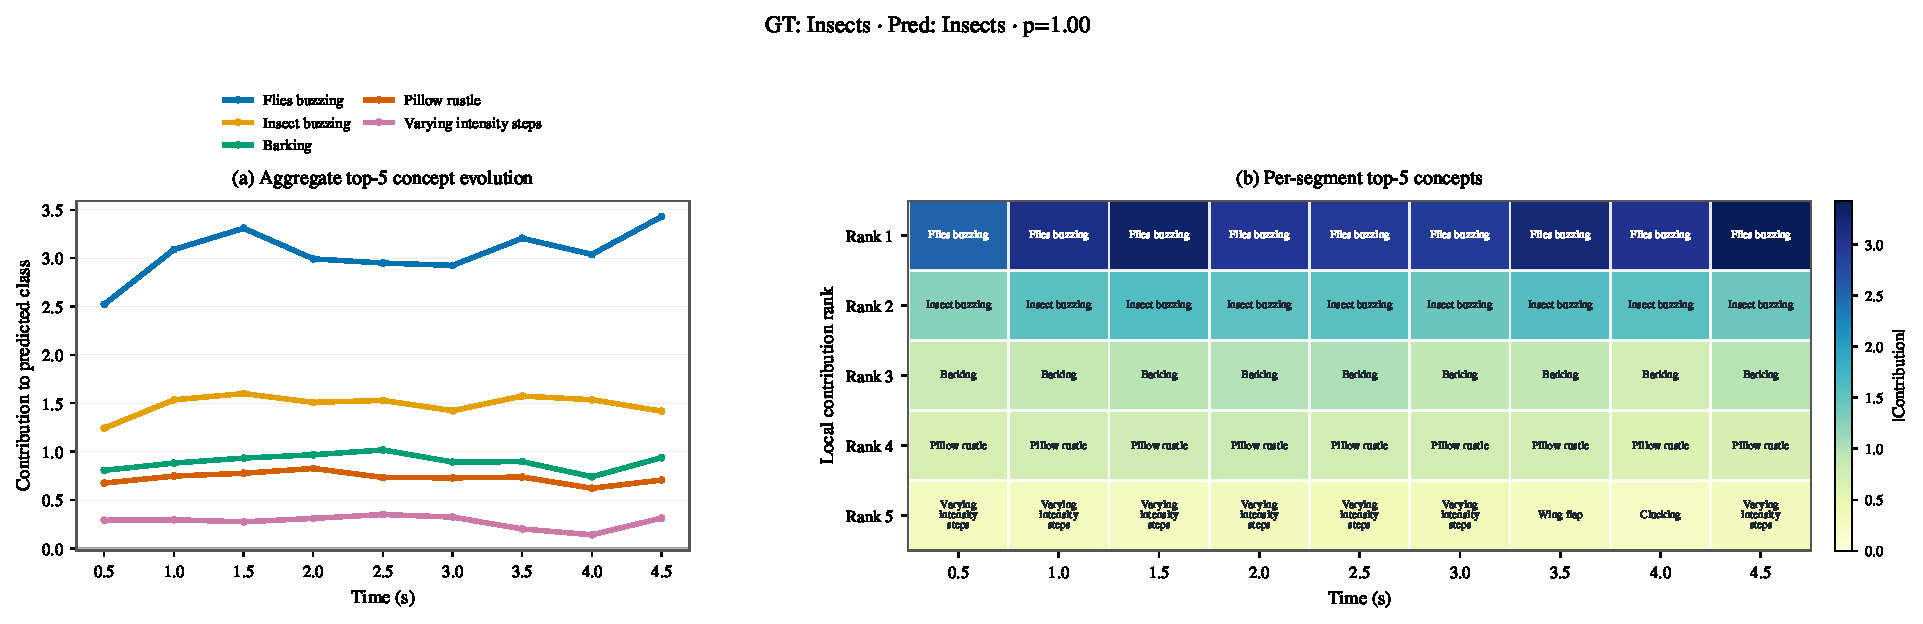
\includegraphics[width=0.43\textwidth]
{media/full_temporal/esc50/02_strongest_correct_1-46938-A-7.pdf} &
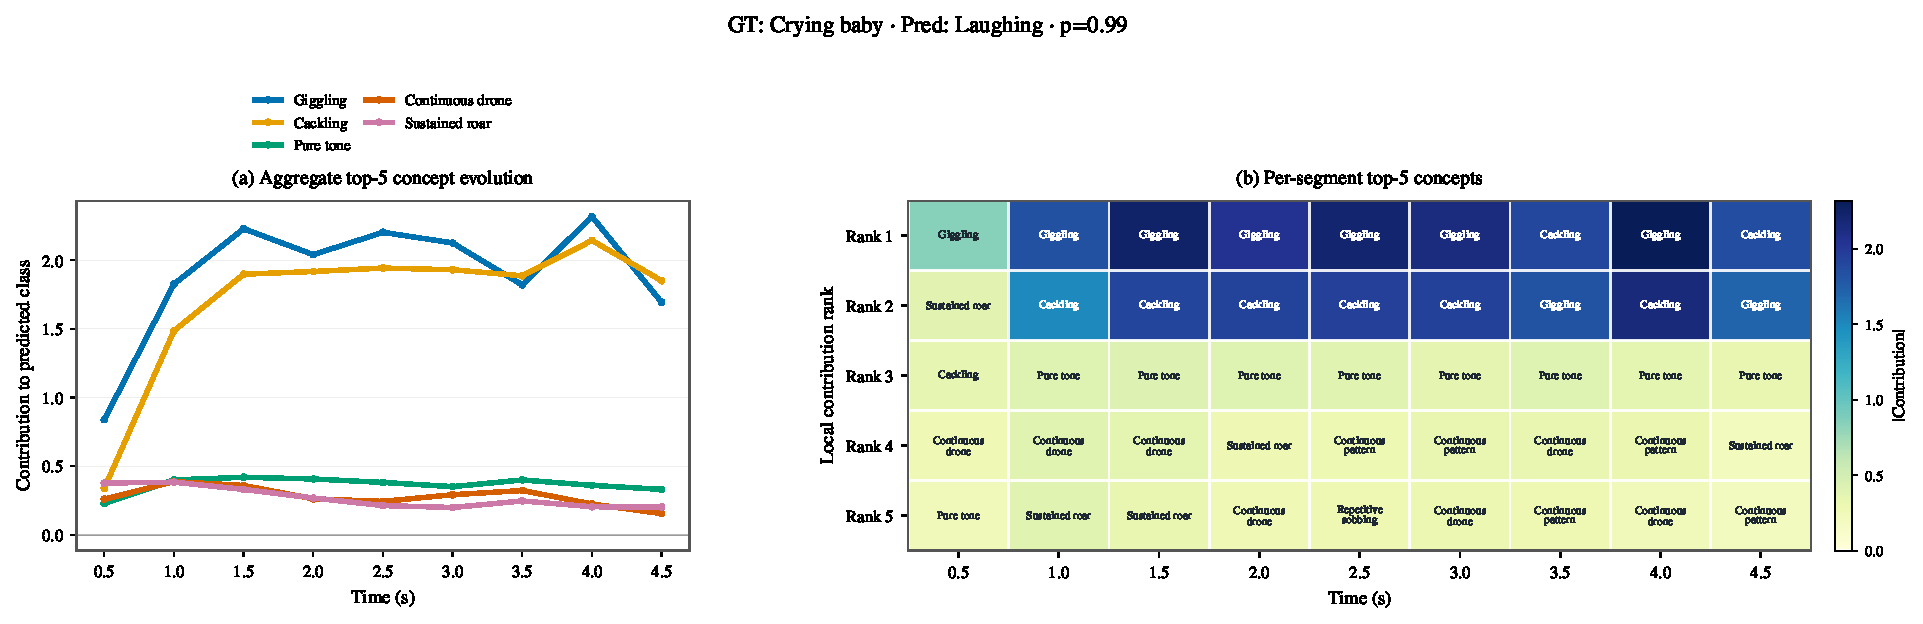
\includegraphics[width=0.43\textwidth]
{media/full_temporal/esc50/01_most_confident_incorrect_1-211527-B-20.pdf}
\end{tabular}

\caption{ESC-50 temporal explanations across concept-generation strategies. Both columns hold the recording fixed across vocabularies: a correctly classified \emph{insects} example (left) and a \emph{crying baby}$\rightarrow$\emph{laughing} failure (right).}
\label{fig:temporal_vocab_esc50}
\end{figure*}


\begin{figure*}[p]
\centering
\setlength{\tabcolsep}{3pt}

\begin{tabular}{@{}c c c@{}}
& \textbf{Correct prediction} & \textbf{Incorrect prediction} \\[0.3em]

\textbf{LF} &

\includegraphics[width=0.43\textwidth]
{media/lf_temporal/urbansound8k/01_strongest_correct_202334-9-0-106.pdf} &

\includegraphics[width=0.43\textwidth]
{media/lf_temporal/urbansound8k/01_most_confident_incorrect_77927-3-1-1.pdf}
\\[0.7em]

\textbf{LF + broad} &

\includegraphics[width=0.43\textwidth]
{media/lf_broad_temporal/urbansound8k/01_strongest_correct_202334-9-0-106.pdf} &

\includegraphics[width=0.43\textwidth]
{media/lf_broad_temporal/urbansound8k/01_most_confident_incorrect_77927-3-1-1.pdf}
\\[0.7em]

\textbf{LF + contrastive} &
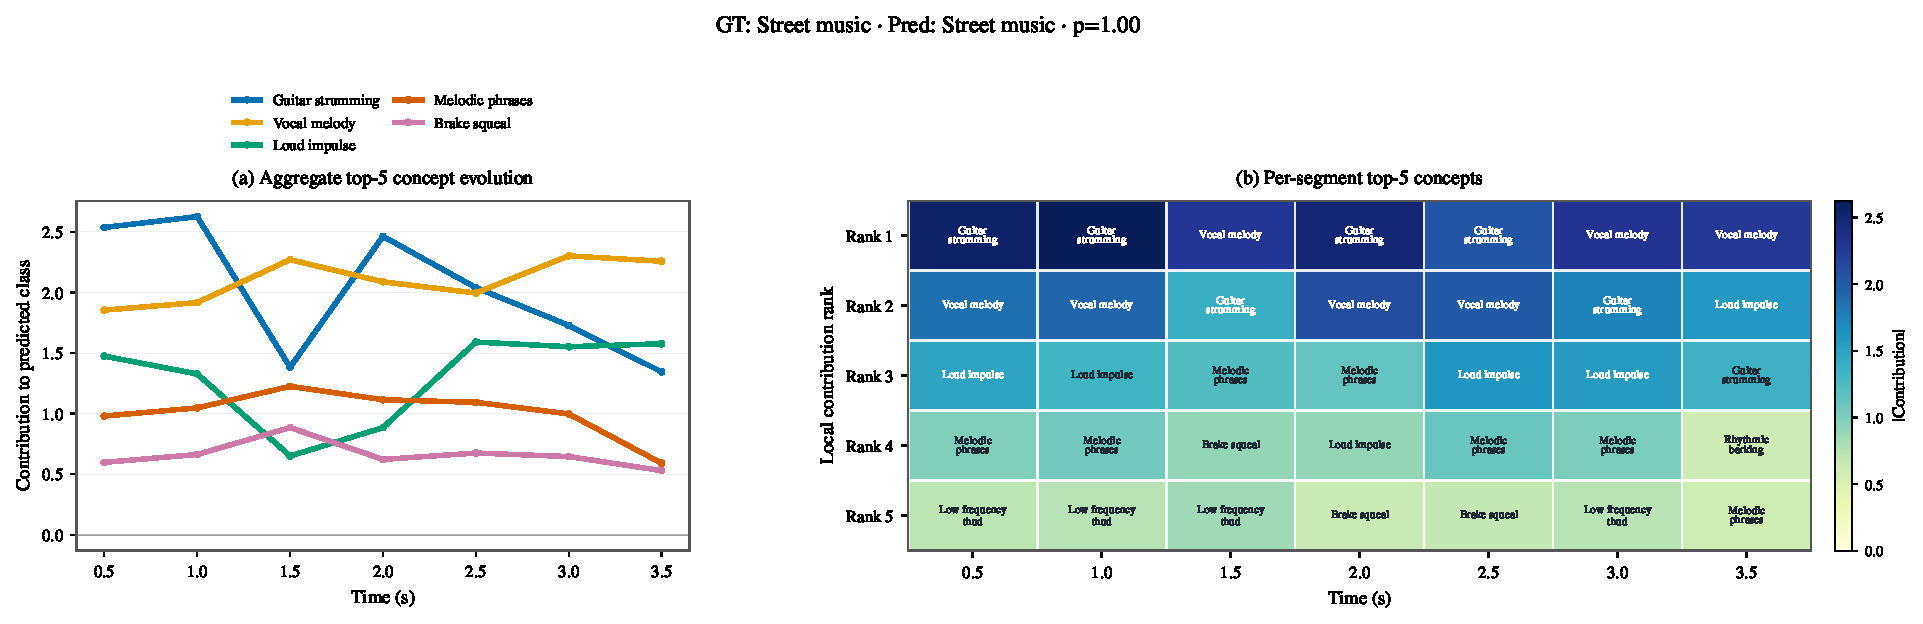
\includegraphics[width=0.43\textwidth]
{media/lf_contrastive_temporal/urbansound8k/01_strongest_correct_155241-9-0-8.pdf} &

\includegraphics[width=0.43\textwidth]
{media/lf_contrastive_temporal/urbansound8k/01_most_confident_incorrect_77927-3-1-1.pdf}
\\[0.7em]

\textbf{Full union} &
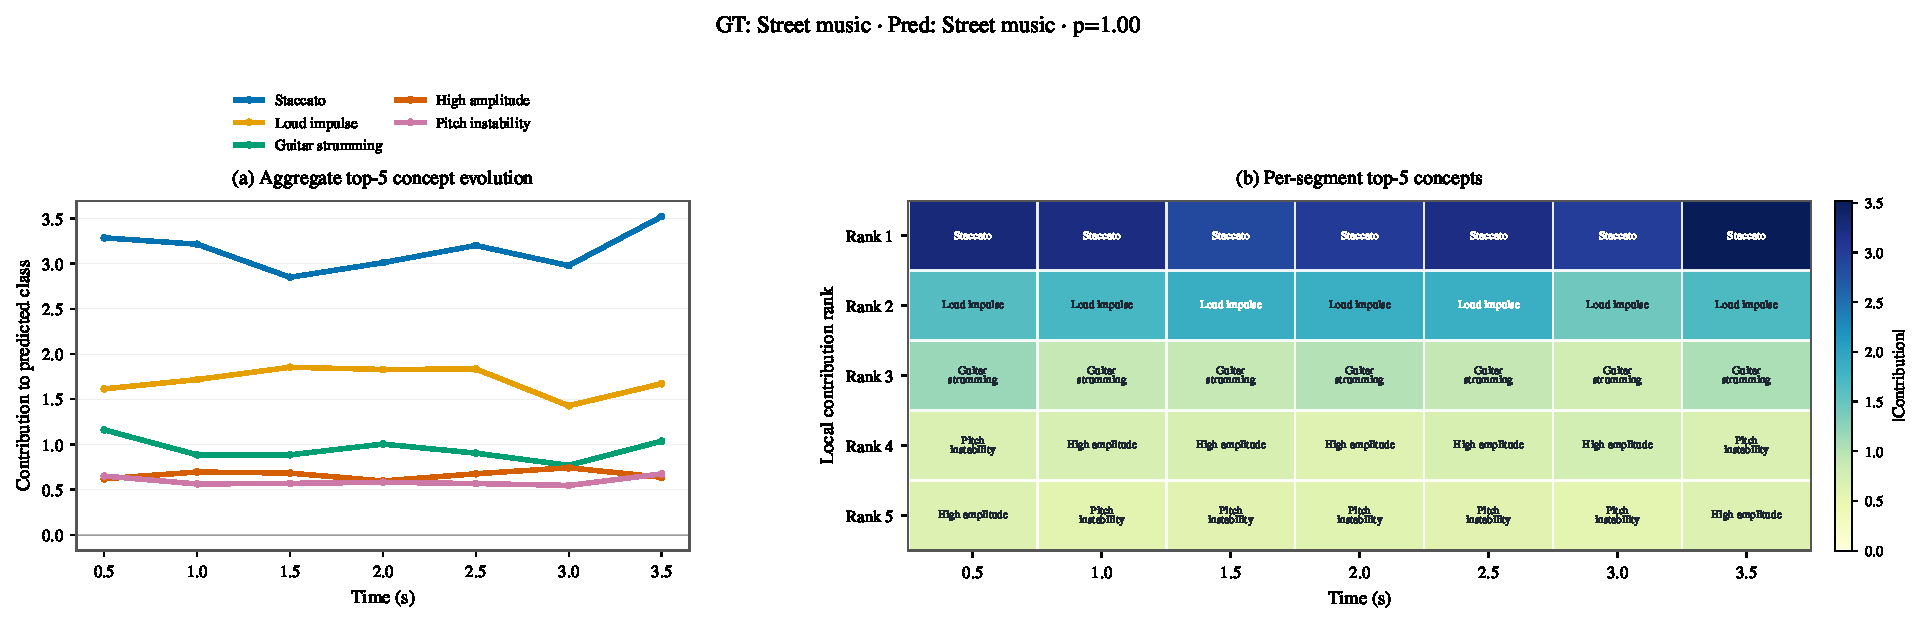
\includegraphics[width=0.43\textwidth]
{media/full_temporal/urbansound8k/01_strongest_correct_202334-9-0-106.pdf} &
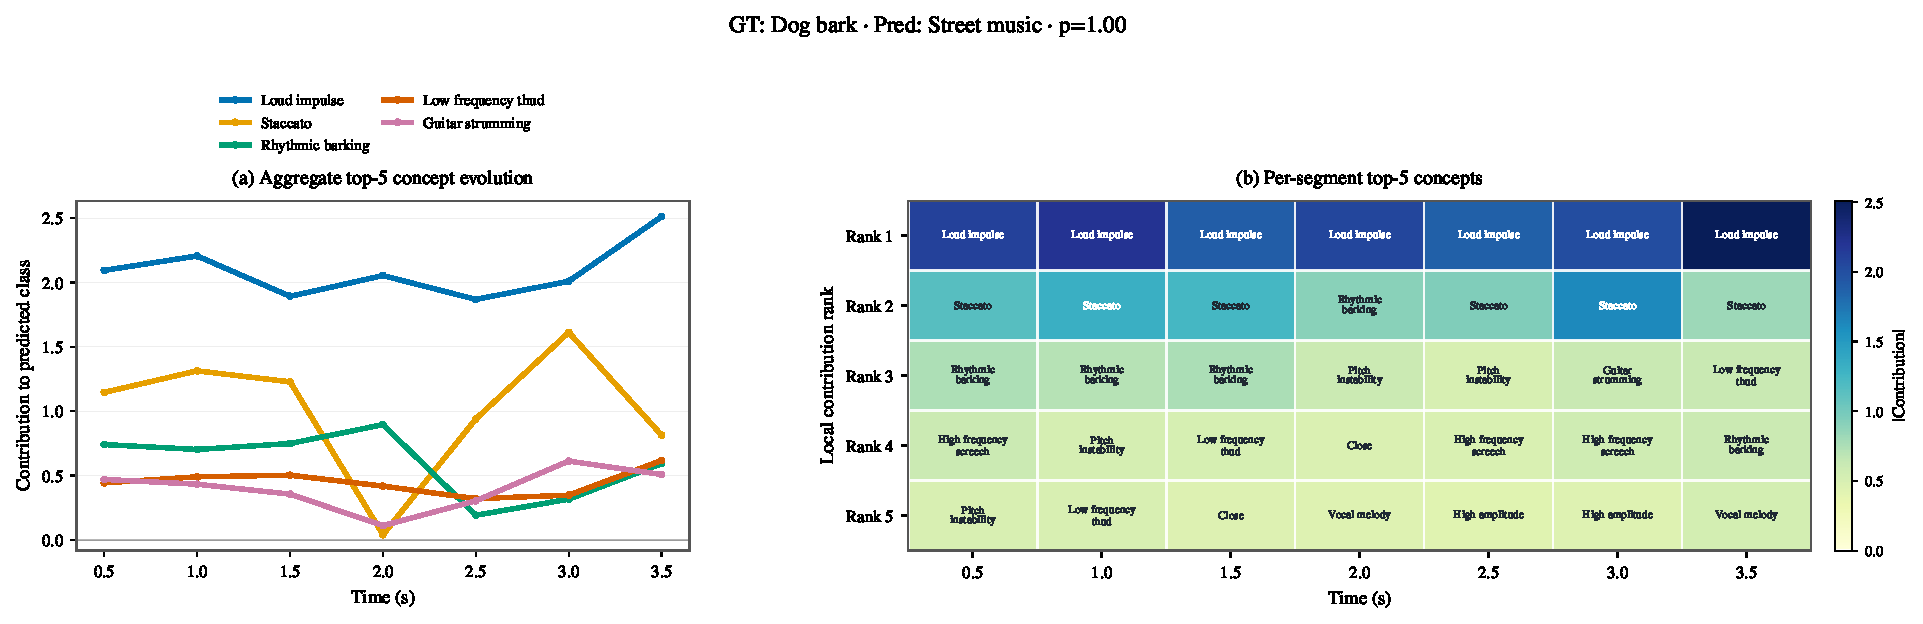
\includegraphics[width=0.43\textwidth]
{media/full_temporal/urbansound8k/01_most_confident_incorrect_77927-3-1-1.pdf}
\end{tabular}

\caption{UrbanSound8K temporal explanations across concept-generation strategies. The left column shows representative high-confidence correct predictions for each vocabulary; the right column holds fixed the same \emph{dog bark}$\rightarrow$\emph{street music} failure (sample 77927-3-1-1), enabling direct comparison of the concepts used to explain the same erroneous decision.}
\label{fig:temporal_vocab_urbansound}
\end{figure*}


\paragraph{CREMA-D qualitative scope.}
The prior CREMA-D figures are not reproduced here because they were generated with the superseded shared vocabulary. The latest speech-targeted study preserves the temporal finding at the quantitative level: targeted full-union inference drops from 70.25/51.58 to 60.58/26.74 under 1-second mean pooling (Table~\ref{tab:segall}), motivating temporal trajectories as a diagnostic rather than a replacement for full-clip prediction.


\paragraph{Summary across concept sources.}
Vanilla LF concepts already recover meaningful temporal evidence, particularly for concrete environmental events. Adding broad concepts improves perceptual readability but can introduce descriptors shared across several classes. Contrastive concepts generally provide more class-specific acoustic evidence and make confusions easier to diagnose. The full union combines both forms of evidence and therefore gives the broadest description, but often at the cost of redundancy or competing cues. Across all variants, the most difficult errors remain acoustically structured rather than arbitrary: the model tends to persistently activate concepts belonging to a plausible but incorrect acoustic family.

\paragraph{Additional correct examples.}
The ESC-50 and UrbanSound8K examples show that the observed structure is not restricted to failures: their LF+broad explanations generally exhibit stable, class-specific acoustic concepts. CREMA-D is discussed under the targeted protocol above rather than mixed with the superseded gallery.

\end{document}
